\chapter{From 0D to 2D}
In solid state physics term of wave vector (remember eq. \ref{eq:wave_fun}) is usually used to describe various materials and their properties. But introducing of wave vector is possible only in case of perfect crystal (without impurities and atoms displacements) and when periodic boundary conditions are enforced. This situation is quit far from reality. So I decided to check, if it is legitimate approximation for real-world crystals.

First I took small piece of graphene zigzag nanoribbon of width $8$ atoms and fixed length $n$. I didn't introduce periodicity in any dimension. I calculated eigen energies of such a system. Density of states of such $0D$ system looks like a set of delta functions. I broadened a bit each energy line and compared density of states for such flakes of graphene of various lengths (fig. \ref{fig:zz_chain}).

It's easy to notice, that density of states for piece of graphene nanoribbon with length $n=200$ looks exactly like DOS for 1D graphene nanoribbon (fig. \ref{fig:1d_dos}). Length of $n=200$ atoms corresponds to $50 nm$.

Next I increased the width of such graphene flakes. Calculated density of states for graphene zigzag nanoribbons of length $100$ atoms and various widths are placed on fig. \ref{fig:flake}.

\begin{figure}[hb!]
\centering
\begin{subfigure}{.45\textwidth}
  \centering
  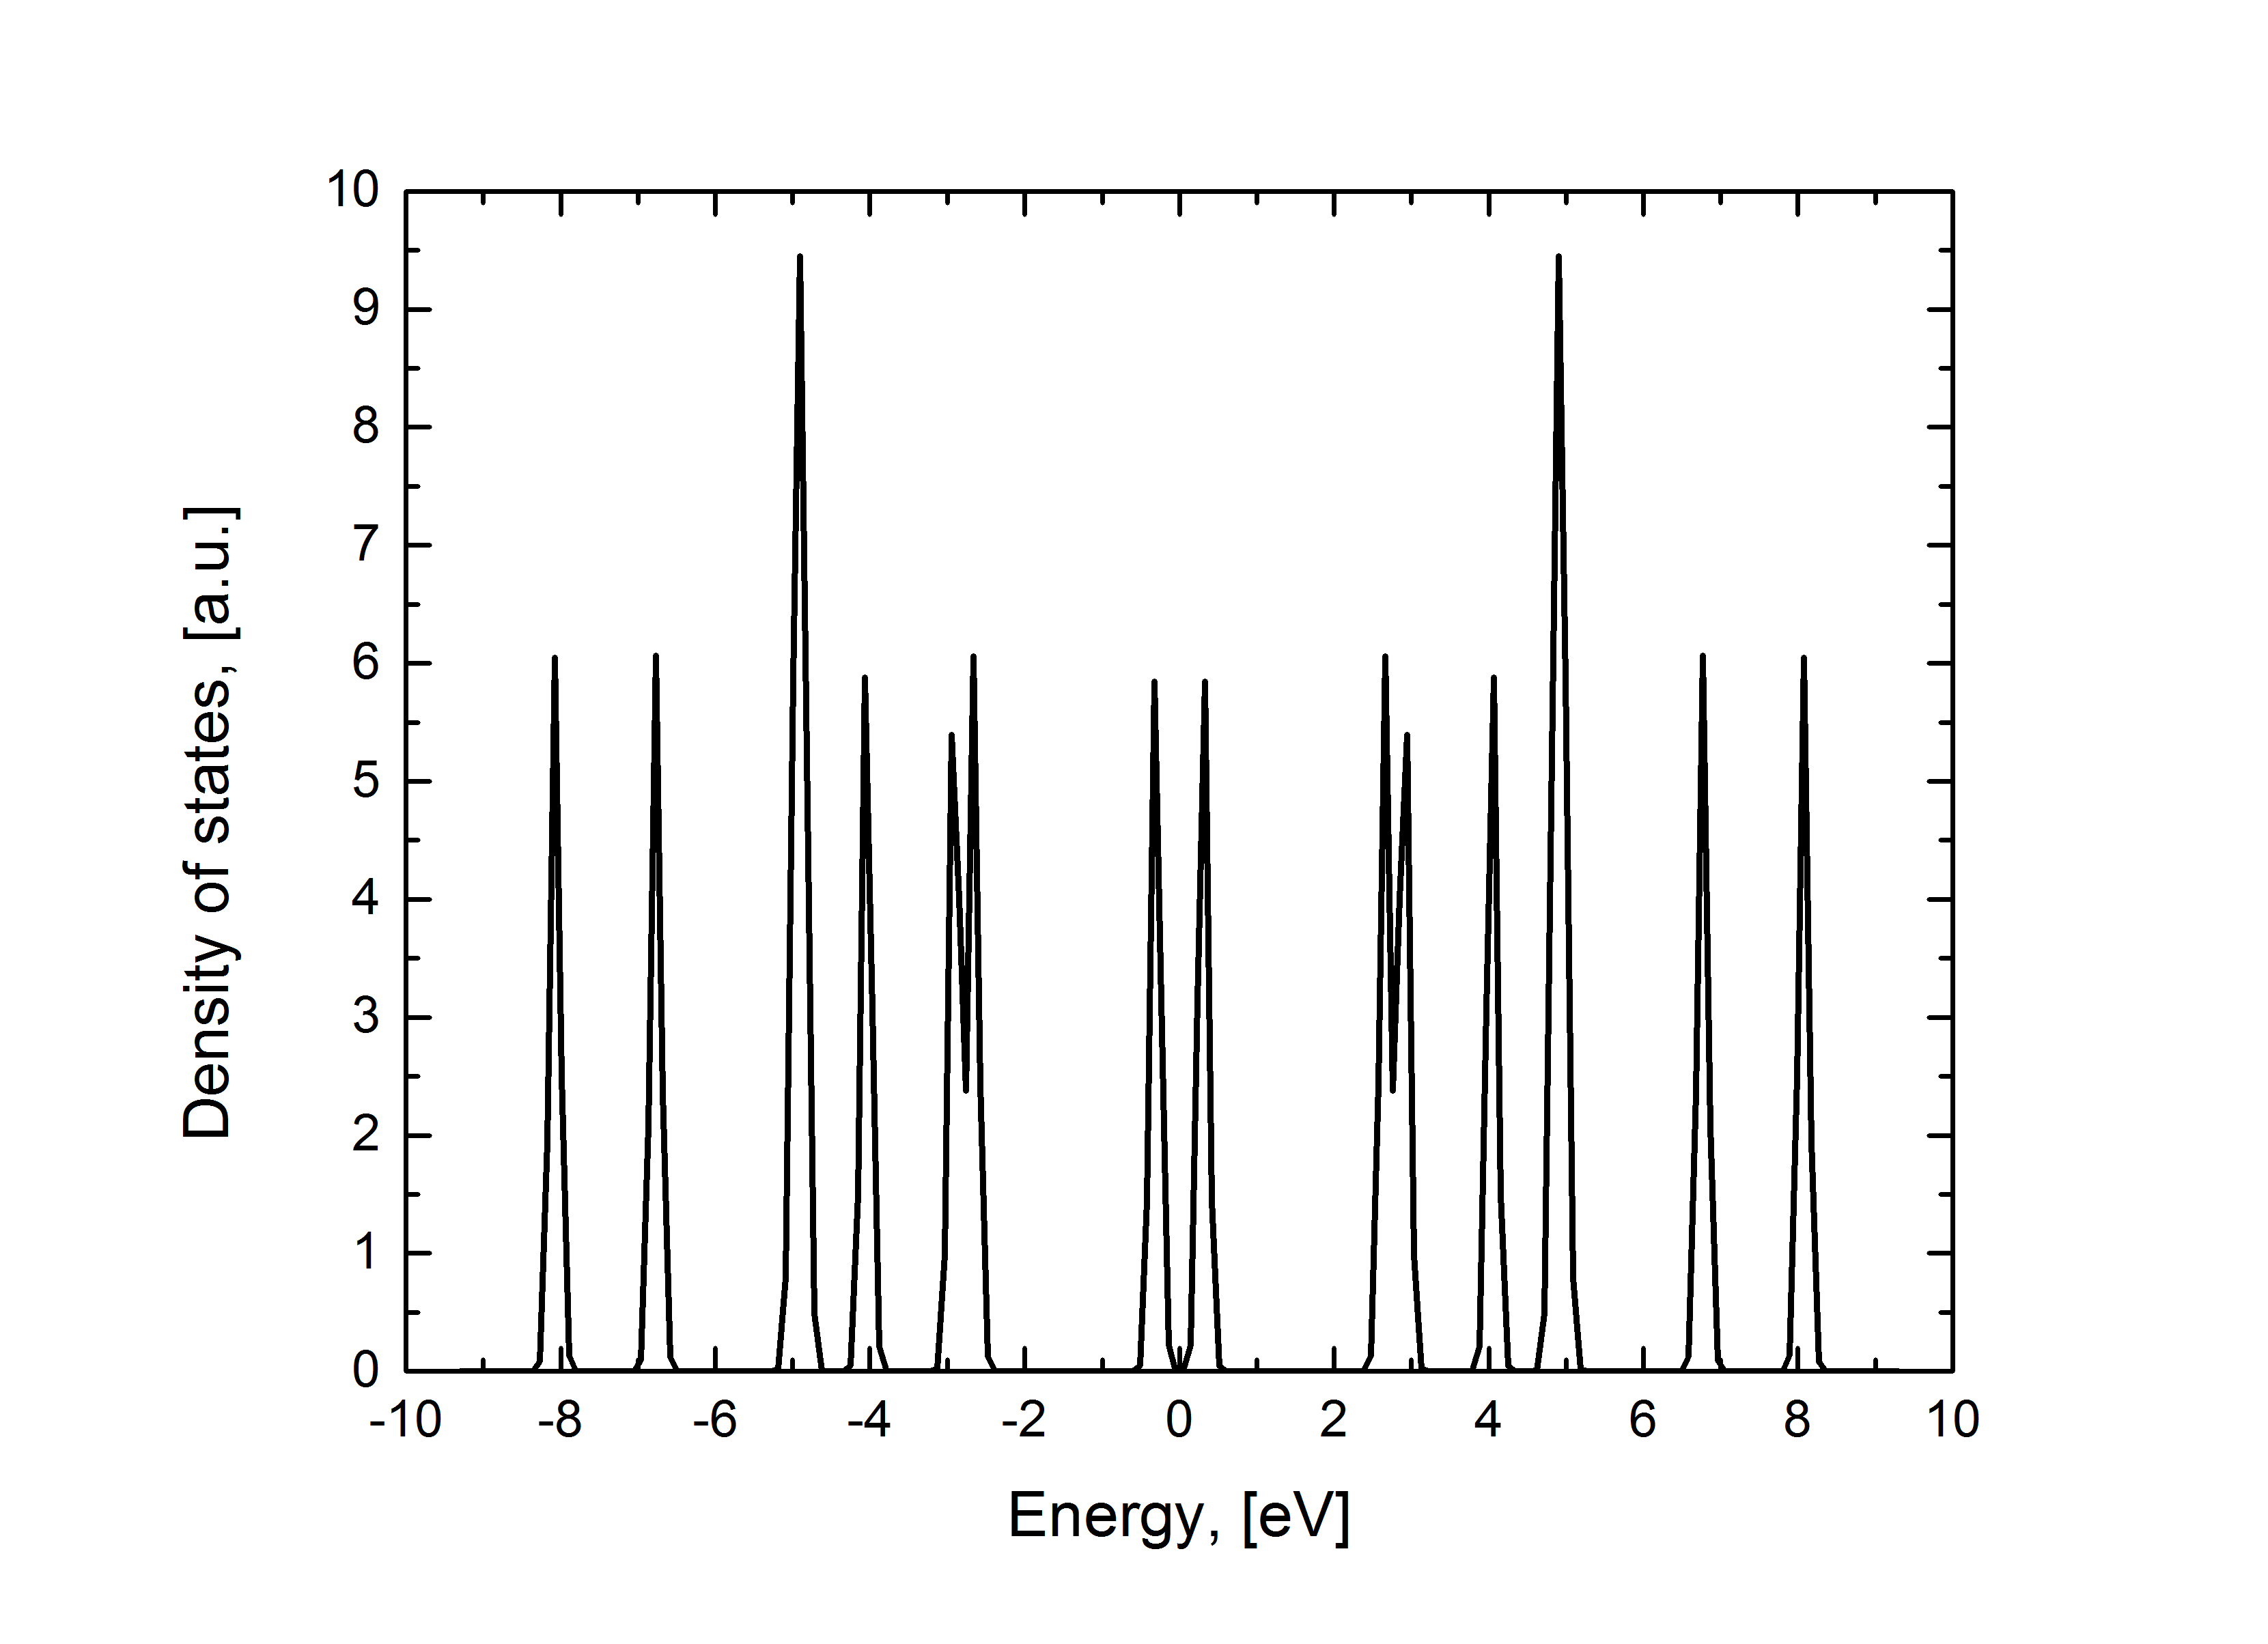
\includegraphics[width=\linewidth]{img/zz_chain_4_dos}
  \caption{$n=4$}
  \label{fig:chain4}
\end{subfigure}%
\begin{subfigure}{.45\textwidth}
  \centering
  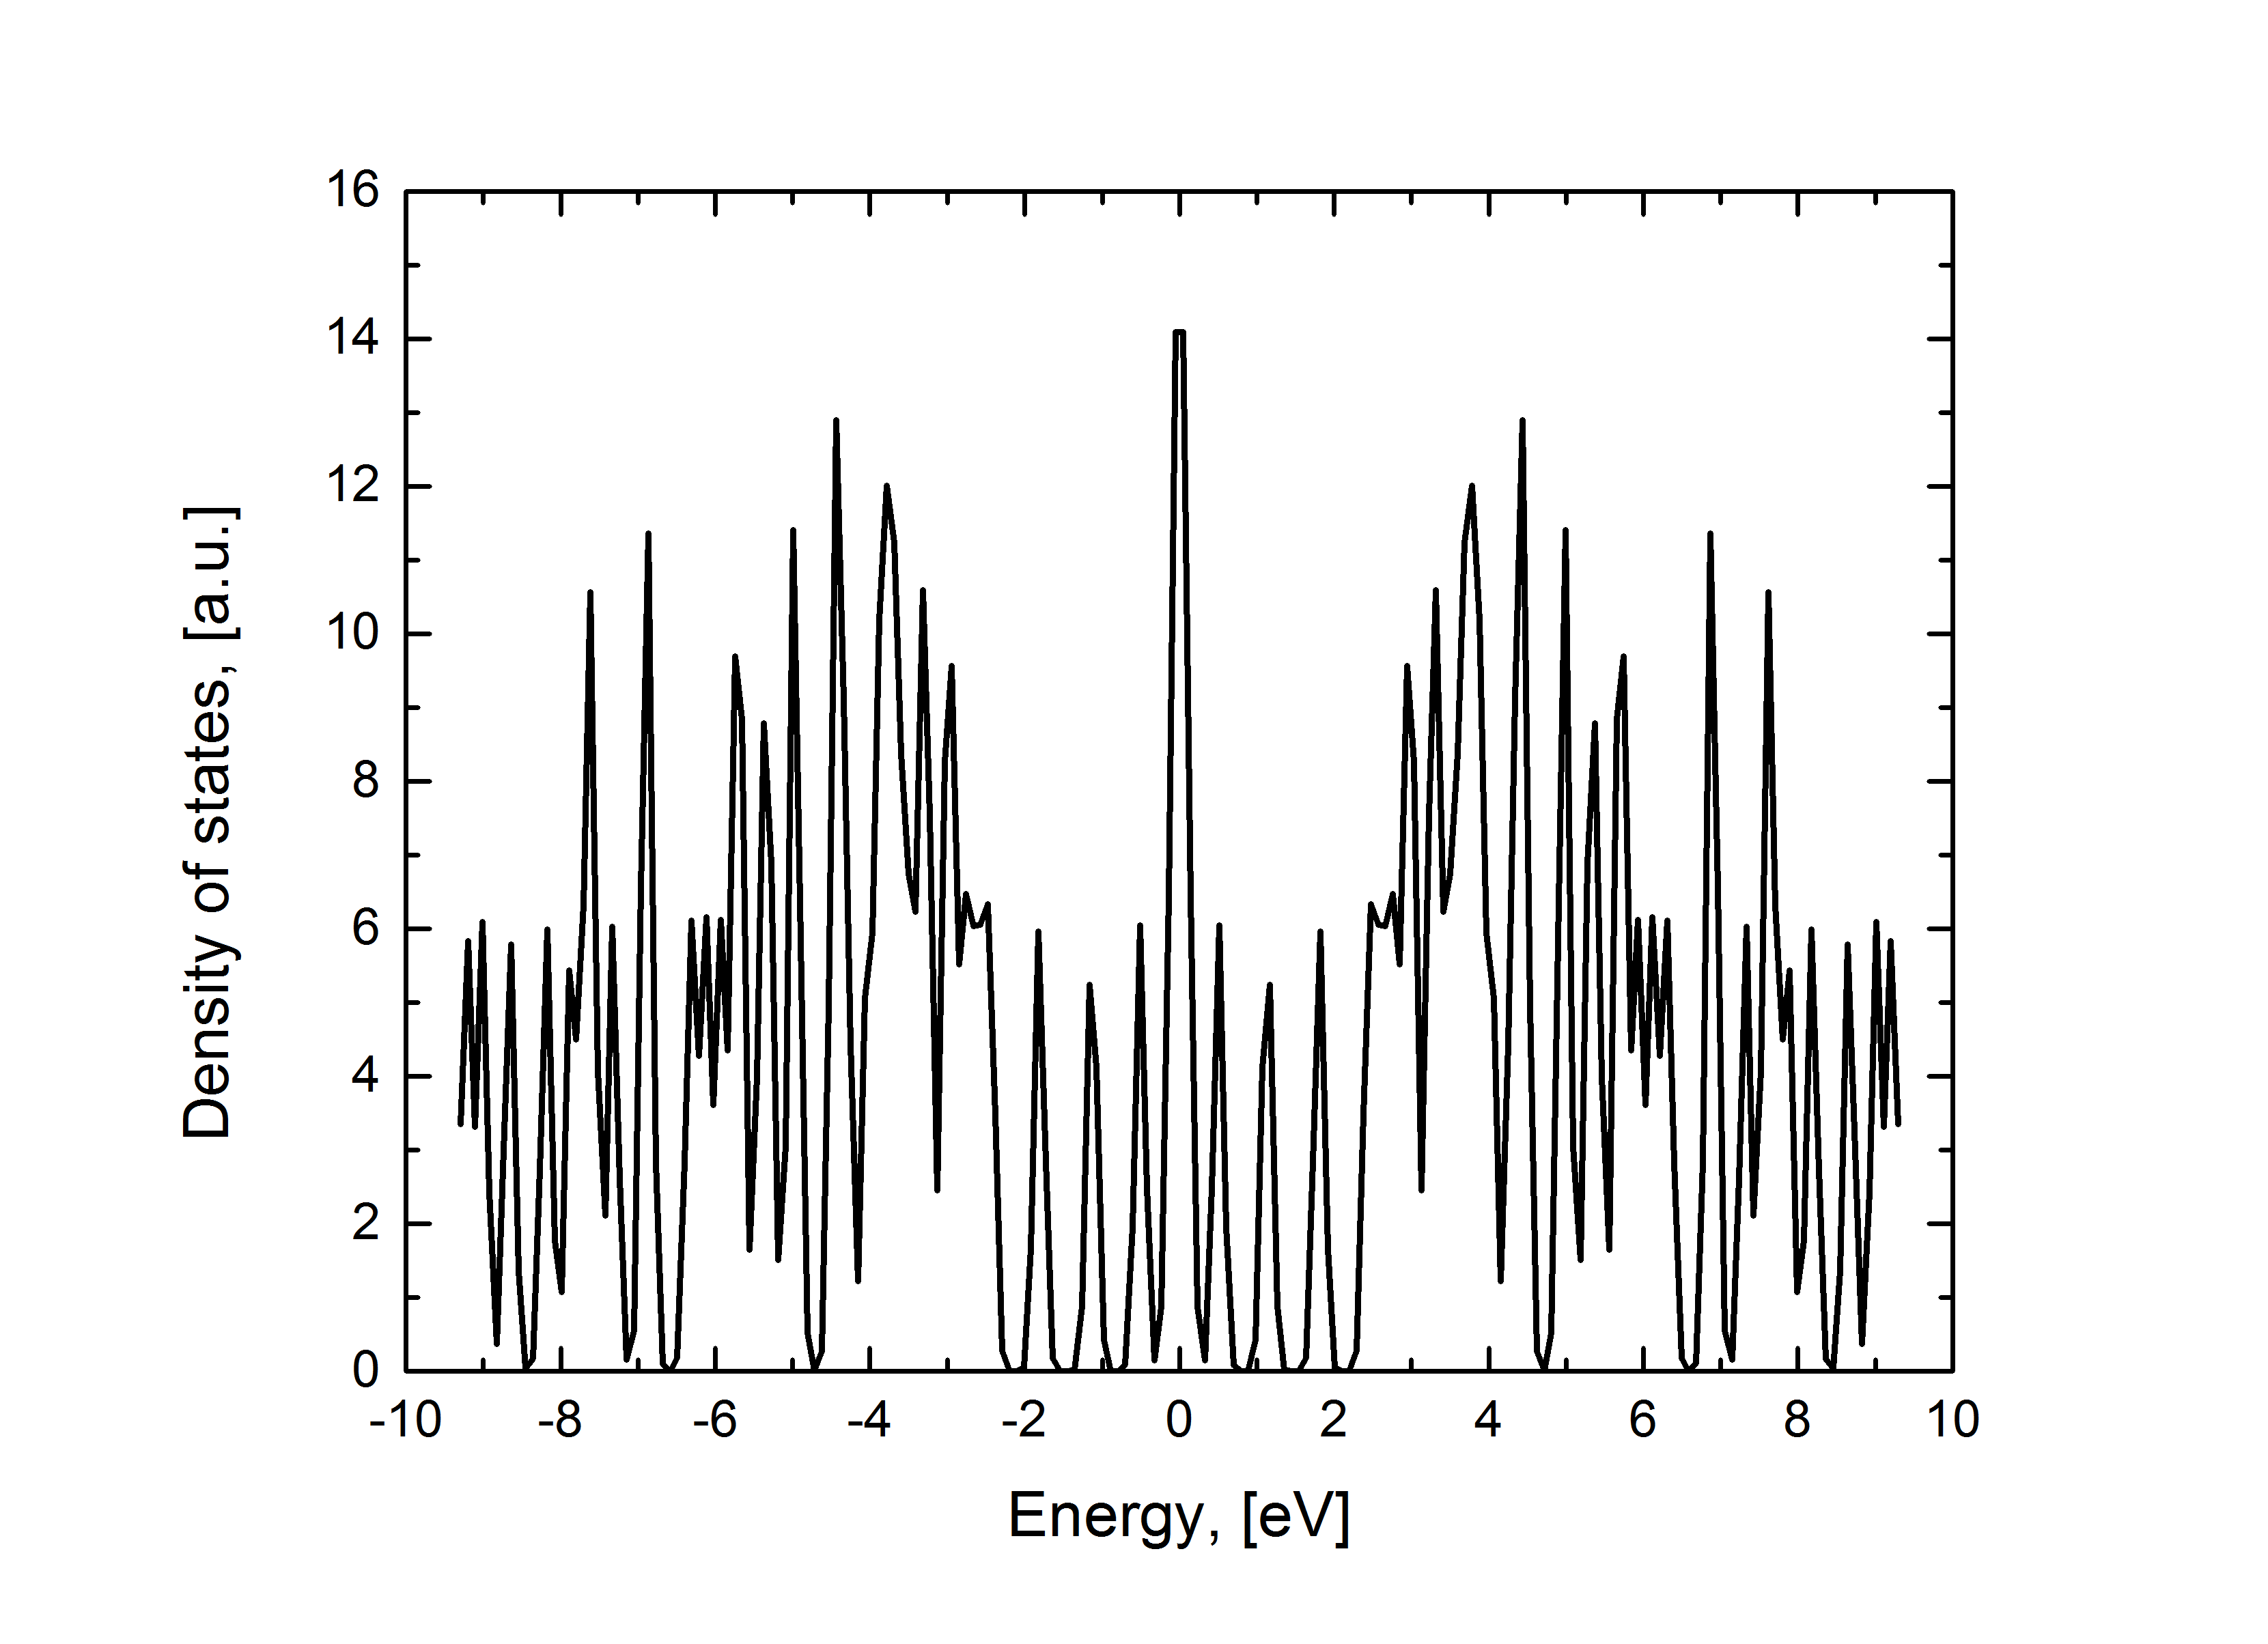
\includegraphics[width=\linewidth]{img/zz_chain_20_dos}
  \caption{$n=20$}
  \label{fig:chain20}
\end{subfigure}
\begin{subfigure}{.45\textwidth}
  \centering
  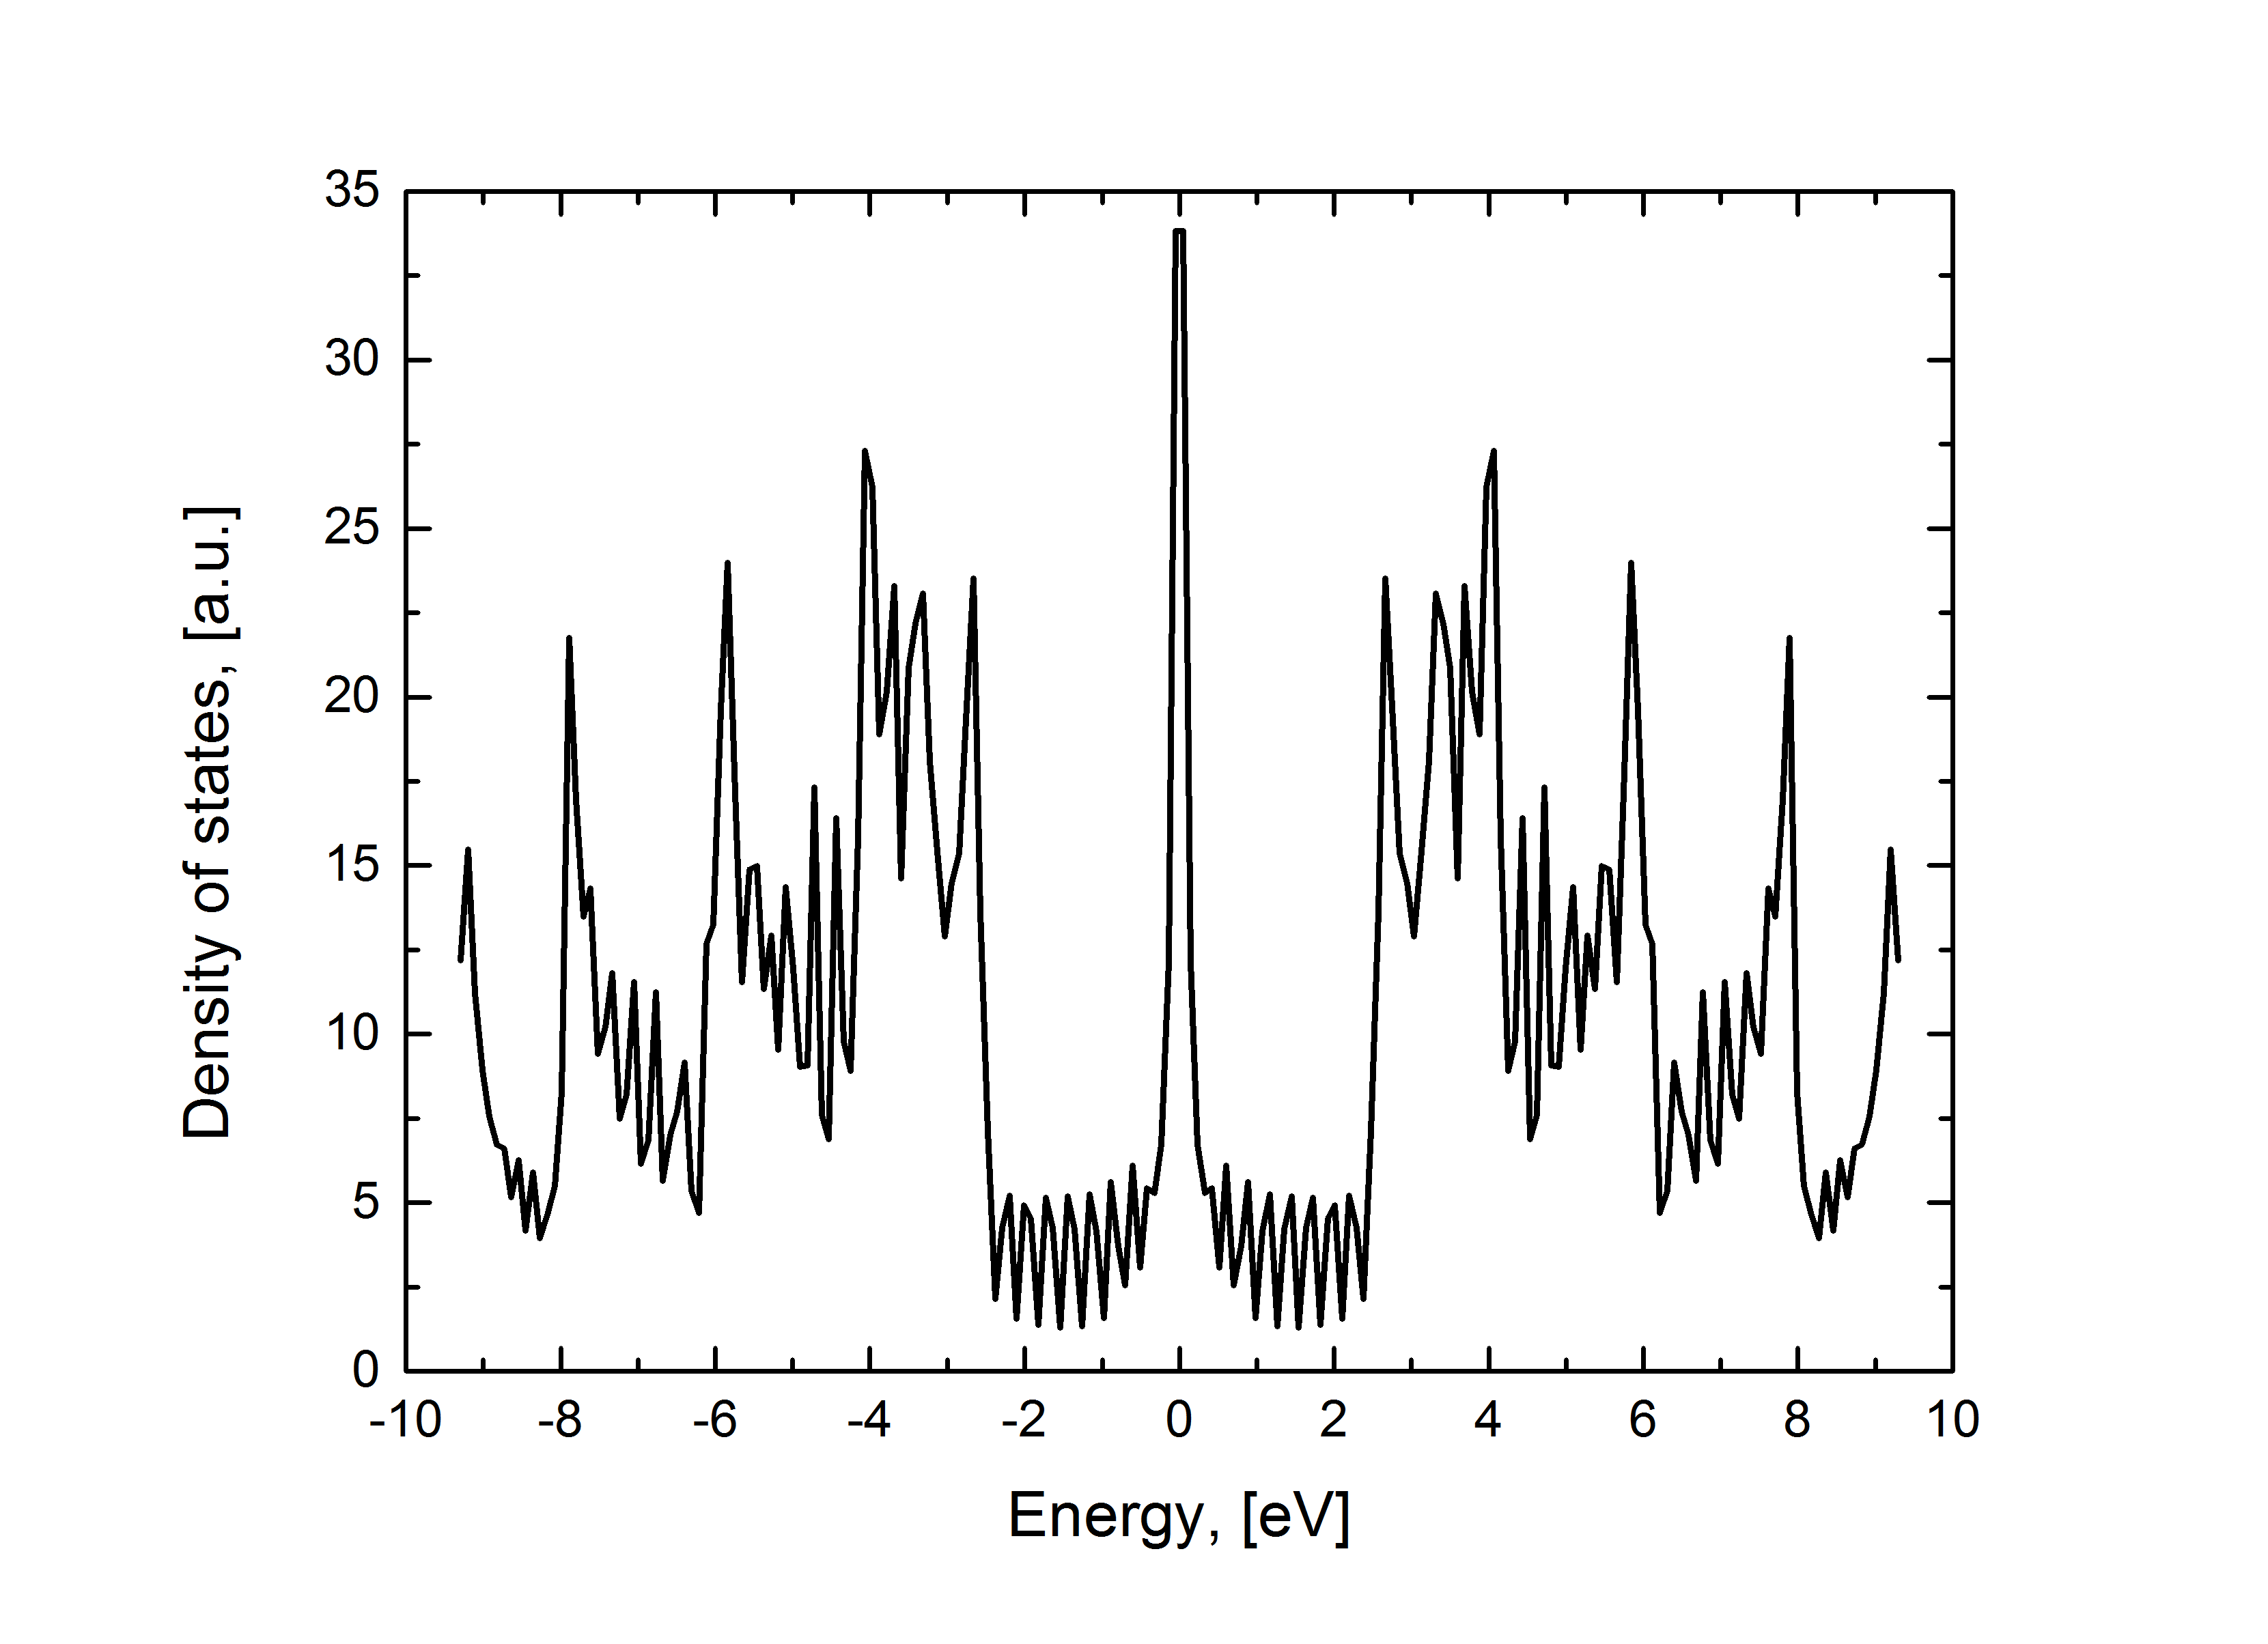
\includegraphics[width=\linewidth]{img/zz_chain_50_dos}
  \caption{$n=50$}
  \label{fig:chain50}
\end{subfigure}
\begin{subfigure}{.45\textwidth}
  \centering
  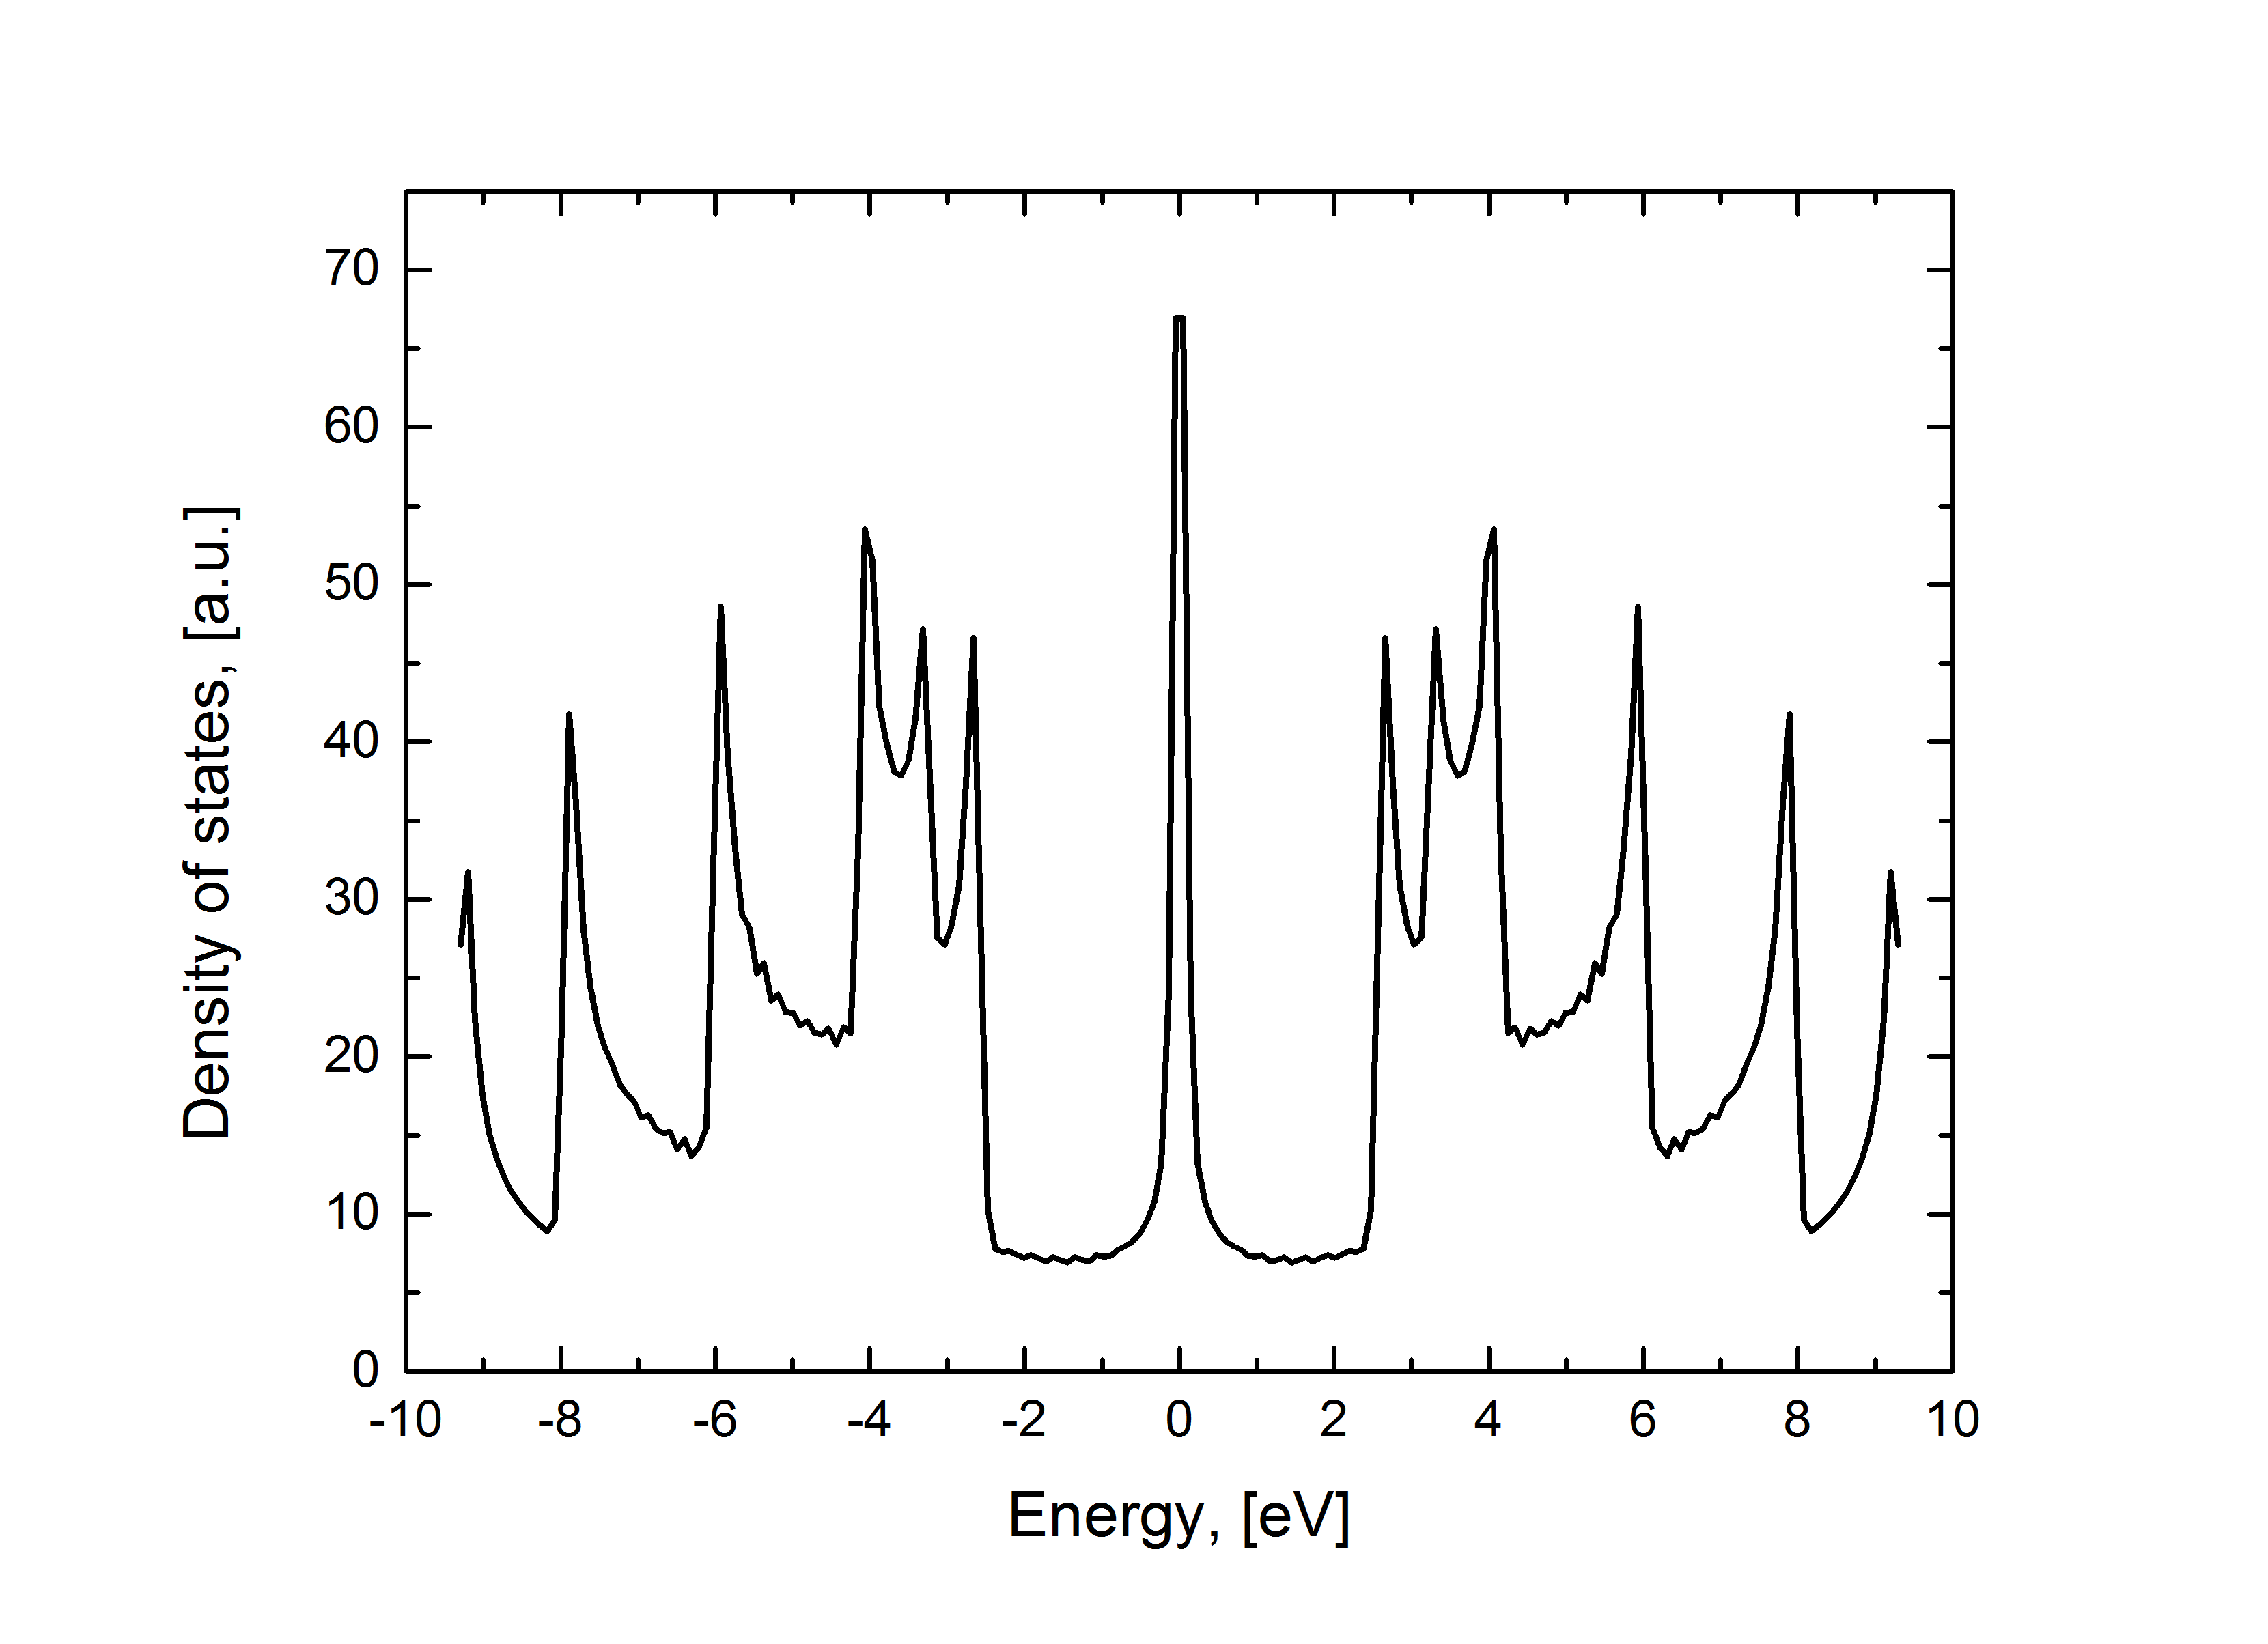
\includegraphics[width=\linewidth]{img/zz_chain_100_dos}
  \caption{$n=100$}
  \label{fig:chain100}
\end{subfigure}
\caption{DOS of pieces of graphene zigzag nanoribbon with width of $8$ atoms and various lengths $n$\label{fig:zz_chain}}
\end{figure}

\begin{figure}[h] 
\begin{center}
  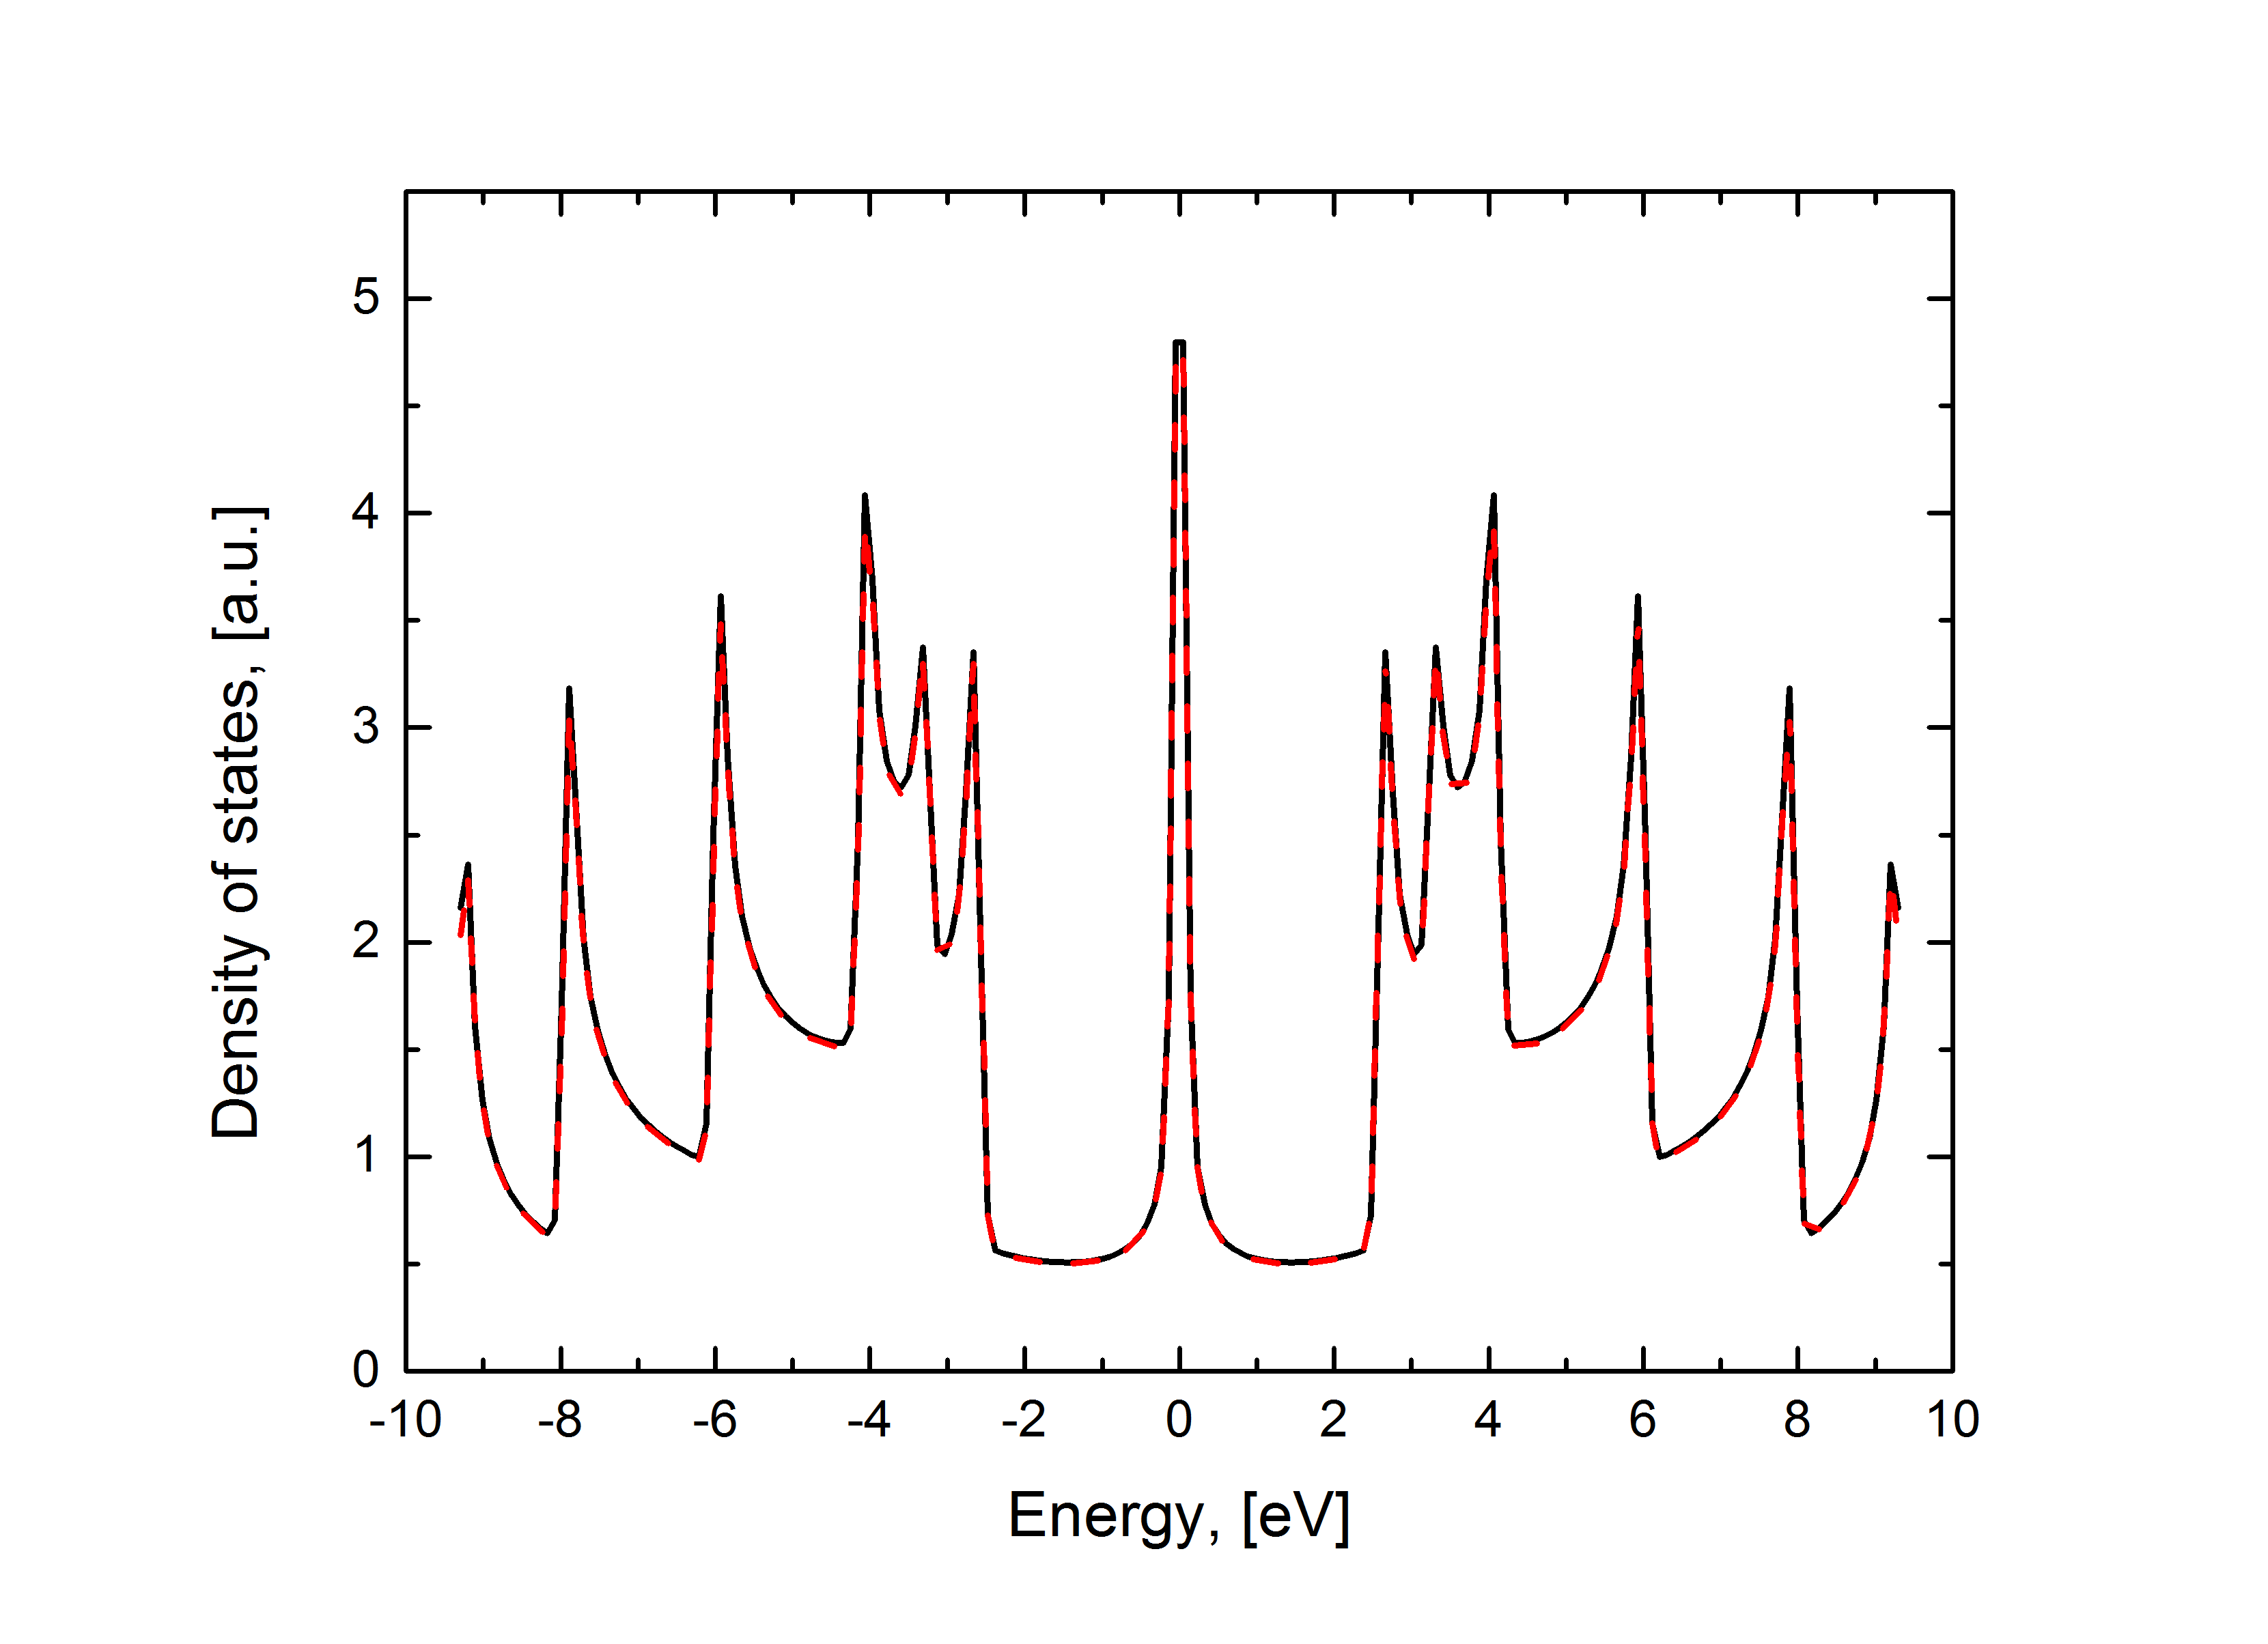
\includegraphics[width=0.6\linewidth]{img/zz_ribbon_2_dos}
  \caption{Black line -- DOS of infinite graphene nanoribbon. Red line -- DOS of graphene nanoribbon of length $n=100$ atoms. \label{fig:1d_dos}}
\end{center}
\end{figure}


\begin{figure}[hb!]
\centering
\begin{subfigure}{.45\textwidth}
  \centering
  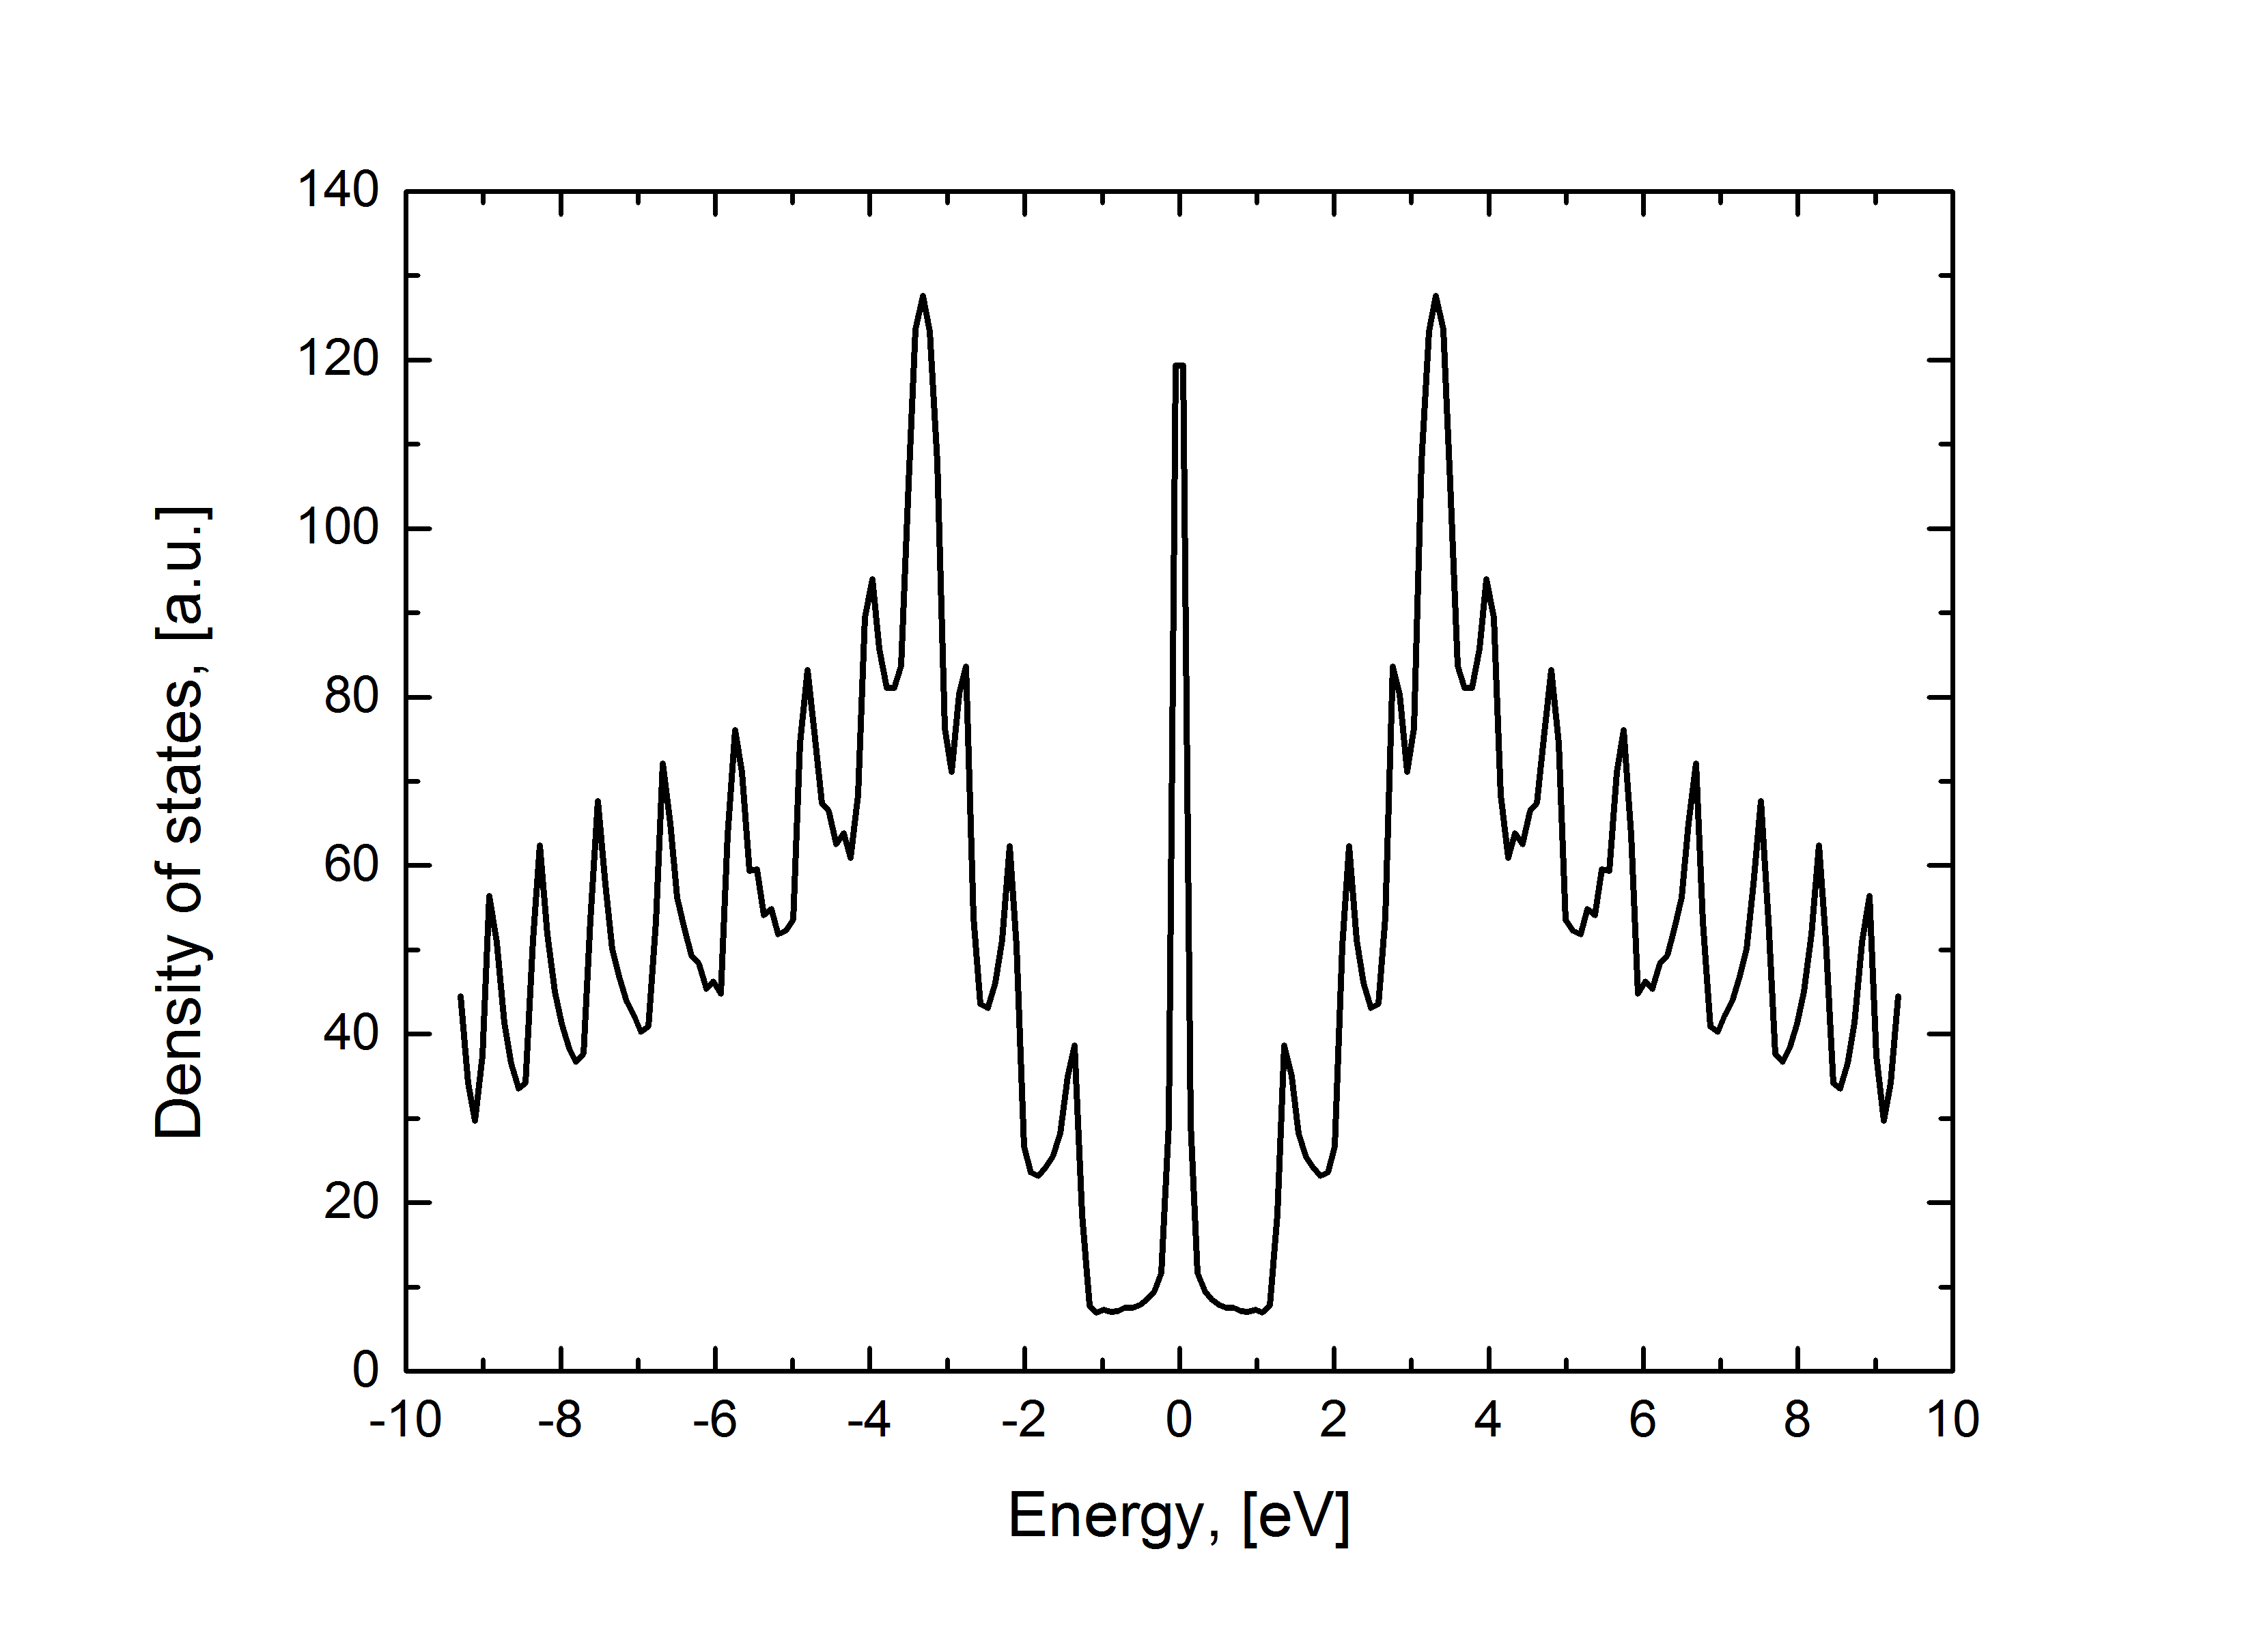
\includegraphics[width=\linewidth]{img/zz_chain_20_100_dos}
  \caption{$n=20$}
  \label{fig:flake20}
\end{subfigure}%
\begin{subfigure}{.45\textwidth}
  \centering
  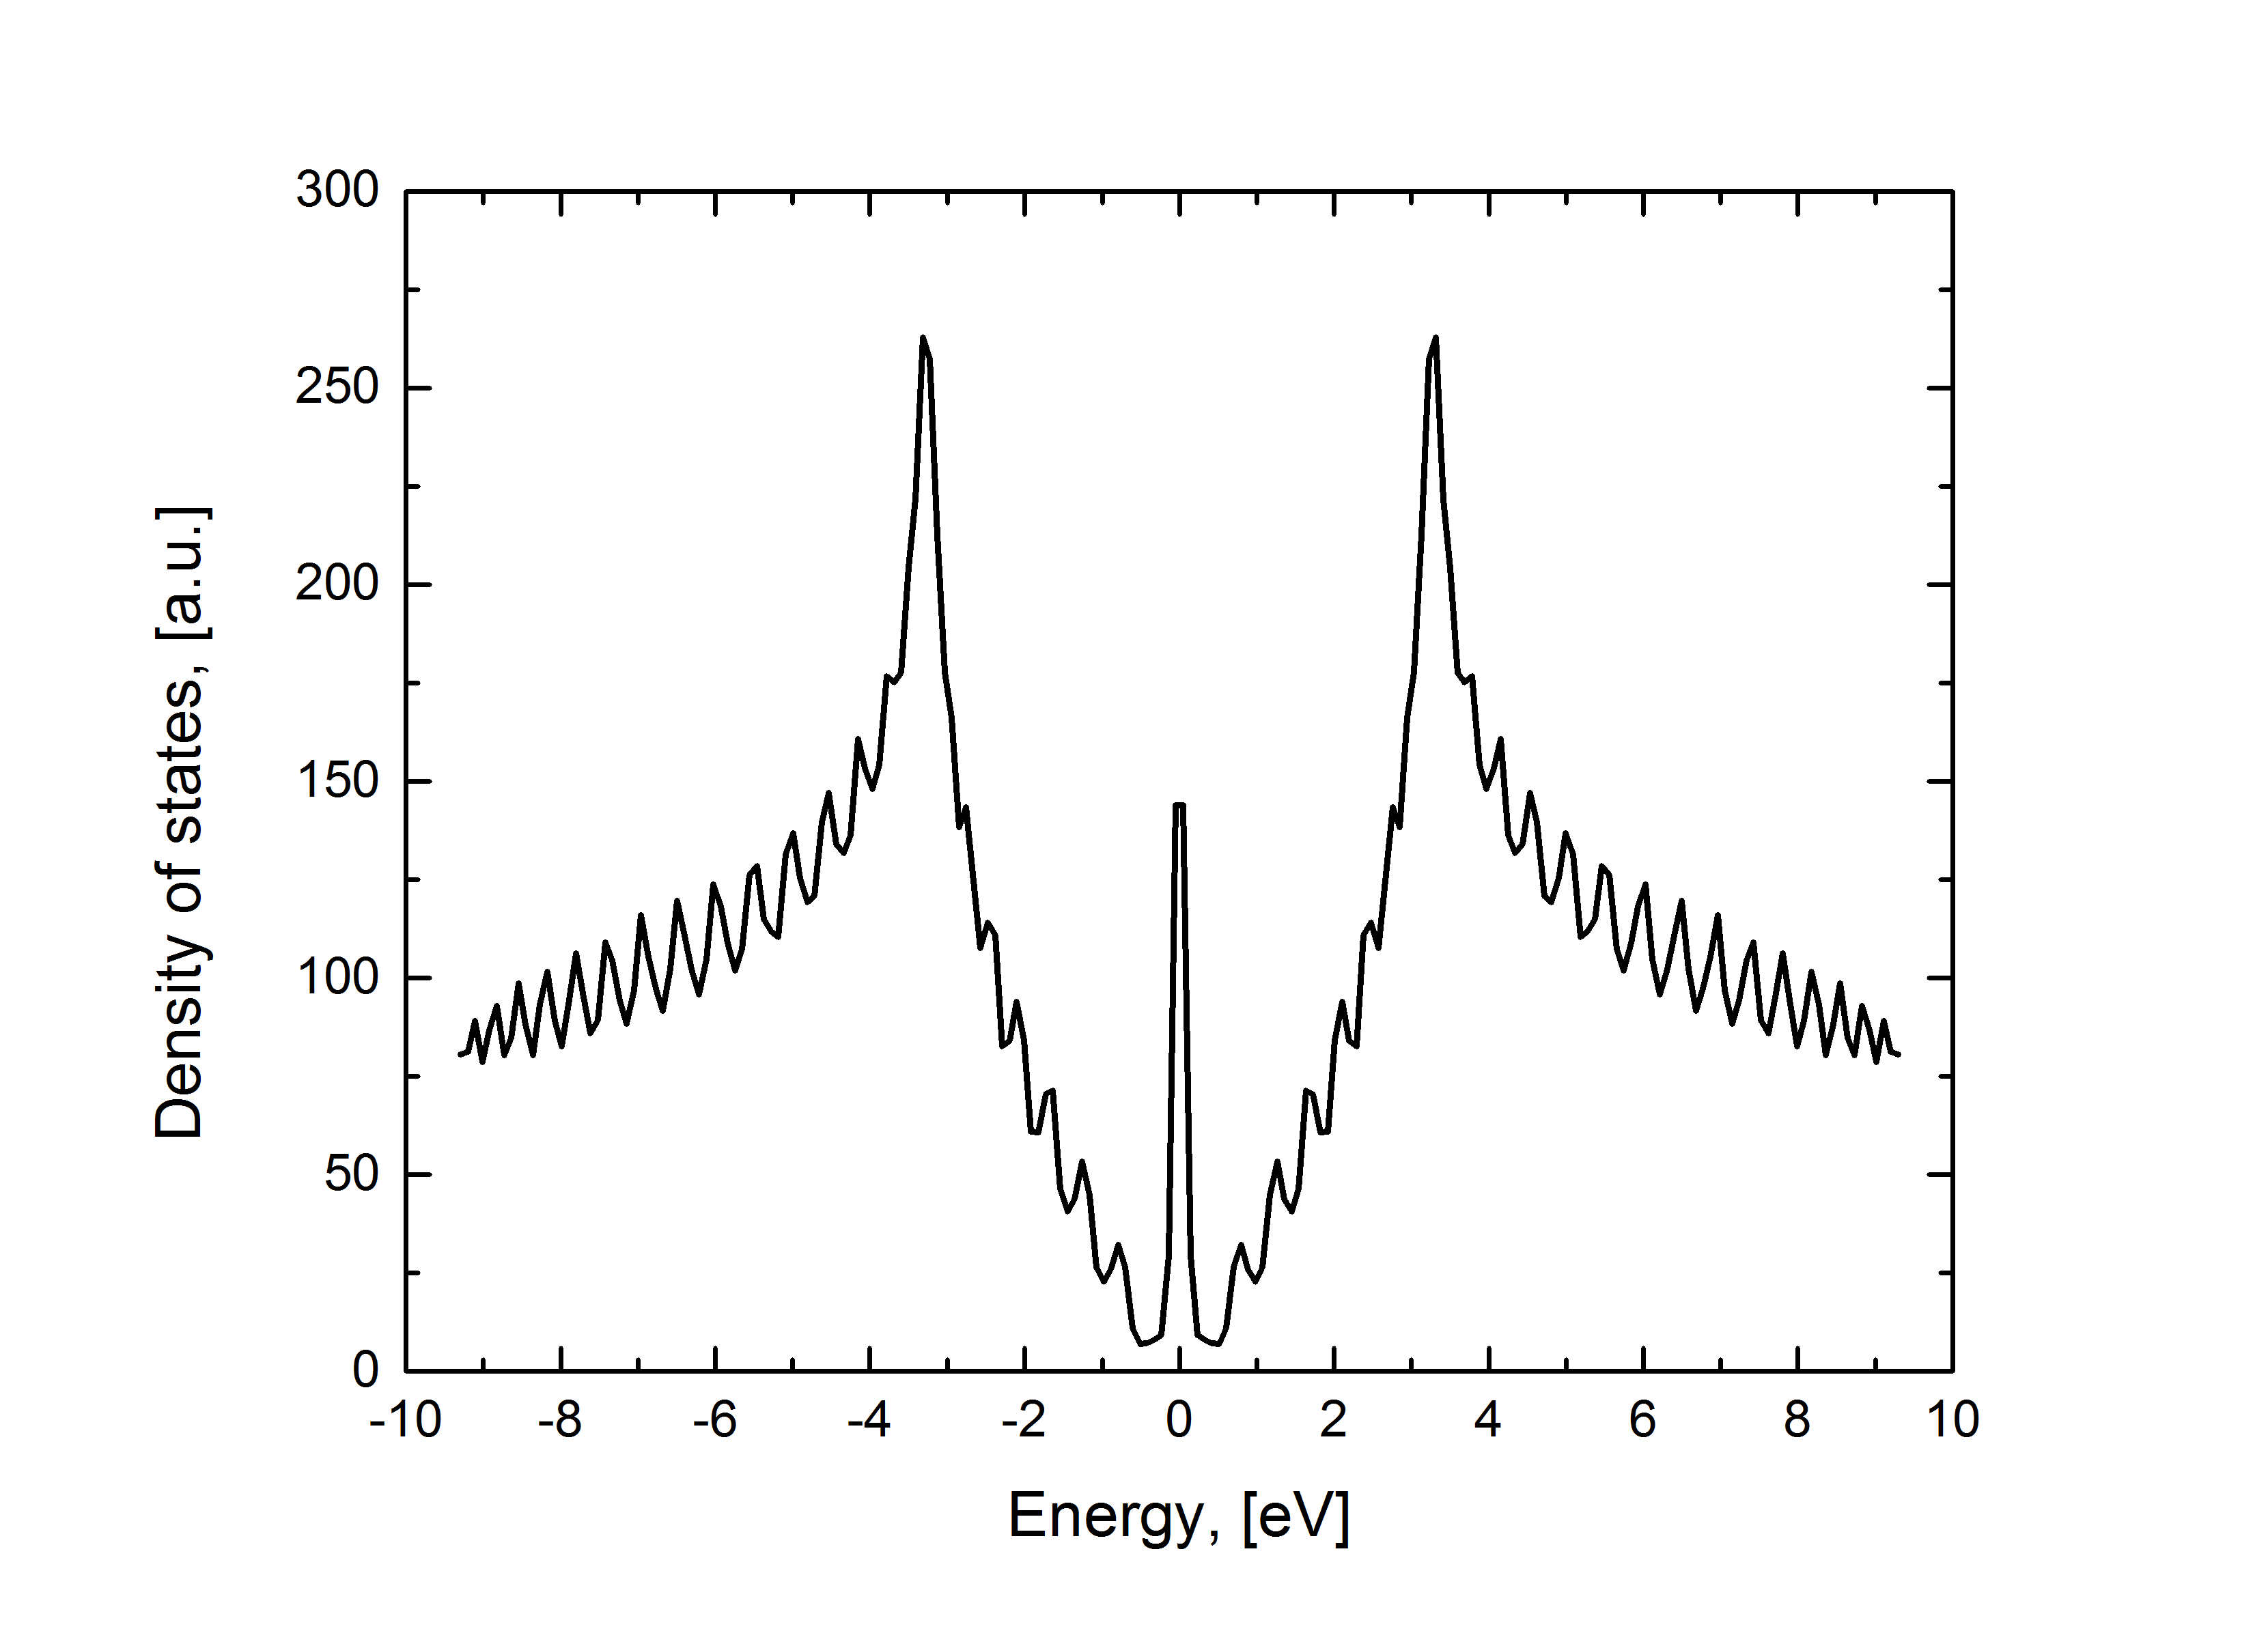
\includegraphics[width=\linewidth]{img/zz_chain_40_100_dos}
  \caption{$n=40$}
  \label{fig:flake40}
\end{subfigure}
\caption{DOS of pieces of graphene zigzag nanoribbon with length of $100$ atoms and various widths $n$\label{fig:flake}}
\end{figure}
